
\begin{figure}[ht]
	\centerline{
\includegraphics[width=0.80\textwidth]{gambar/dapi1.jpg}}
	\caption{Typesetting Math in Latex}
	\label{Typesetting Math in Latex}
\end{figure}


\section {Pengertian }
\subsection {Typesetting Math in Latex}
 \hspace*{0.5in} Latex Adalah Sebuah alat yang sangat kuat untuk typesetting pada umumnya dan untuk typesetting matematika masuk tertentu. Namun, terlepas dari kekuatannya, masih banyak cara untuk menghasilkannya hasil yang lebih baik atau kurang bagus. Panduan ini menawarkan beberapa trik dan petunjuk yang mudah-mudahan akan dilakukan mengarah ke yang pertama Perhatikan bahwa manual ini tidak mengklaim untuk memberikan yang terbaik atau satu-satunya solusi. Tujuannya adalah untuk memberi beberapa aturan yang bisa diikuti dengan mudah dan itu akan memimpin ke tata letak yang baik dari semua persamaan dalam sebuah dokumen. Hal ini diasumsikan bahwa pembaca memiliki sudah menguasai dasar-dasar Latex \par
\noindent 
\hspace*{0.5in} Struktur dokumen ini adalah sebagai berikut. Kami memperkenalkan persamaan yang paling dasar di Bagian 2; Bagian 3 kemudian menjelaskan beberapa kemungkinan reaksi pertama ketika sebuah persamaan terlalu panjang Bagian terpenting dari manual ini tercantum dalam Bagian 4 dan 5: disana kita perkenalkan yang bertenaga IEEEeqnarray lingkungan yang harus digunakan masuk apapun bukan meluruskan atau eqnarray.Dalam Bagian 6 beberapa masalah yang lebih maju dan solusi yang mungkin dibahas, dan Bagian 7 berisi beberapa petunjuk dan trik tentang editor Emacs. Akhirnya, Bagian 8 membuat beberapa saran tentang beberapa simbol matematika khusus yang tidak dapat dengan mudah dadjustwidthukan di Latex. \par
\noindent 
\vspace{12pt}
\noindent 
\vspace{12pt}
\noindent 


\subsection{Bagaimana~persamaan typeset di  Sebuah Latex file sumber dari manual ini.}


\begin{enumerate}



\item  dot : perintah untuk disertakan dalam file preferensi Emacs (.emacs) 
\item IEEEtrantool [2015/08/26 V1.5 oleh Michael Shell]: paket yang dibutuhkan untuk IEEEeqnarray-lingkungan Hidup. 
\item IEEEtran [2015/08/26 V1.8b oleh Michael Shell]: Latex dalam format IEEE. 
\item  manual resmi dari IEEEtran-kelas. Bagian tentang IEEEeqnarray dadjustwidthukan di Appendix F. Perhatikan itu IEEEtran.cls dan IEEEtrantools.sty disediakan secara otomatis oleh siapapun up-to-date.\

\end {enumerate}

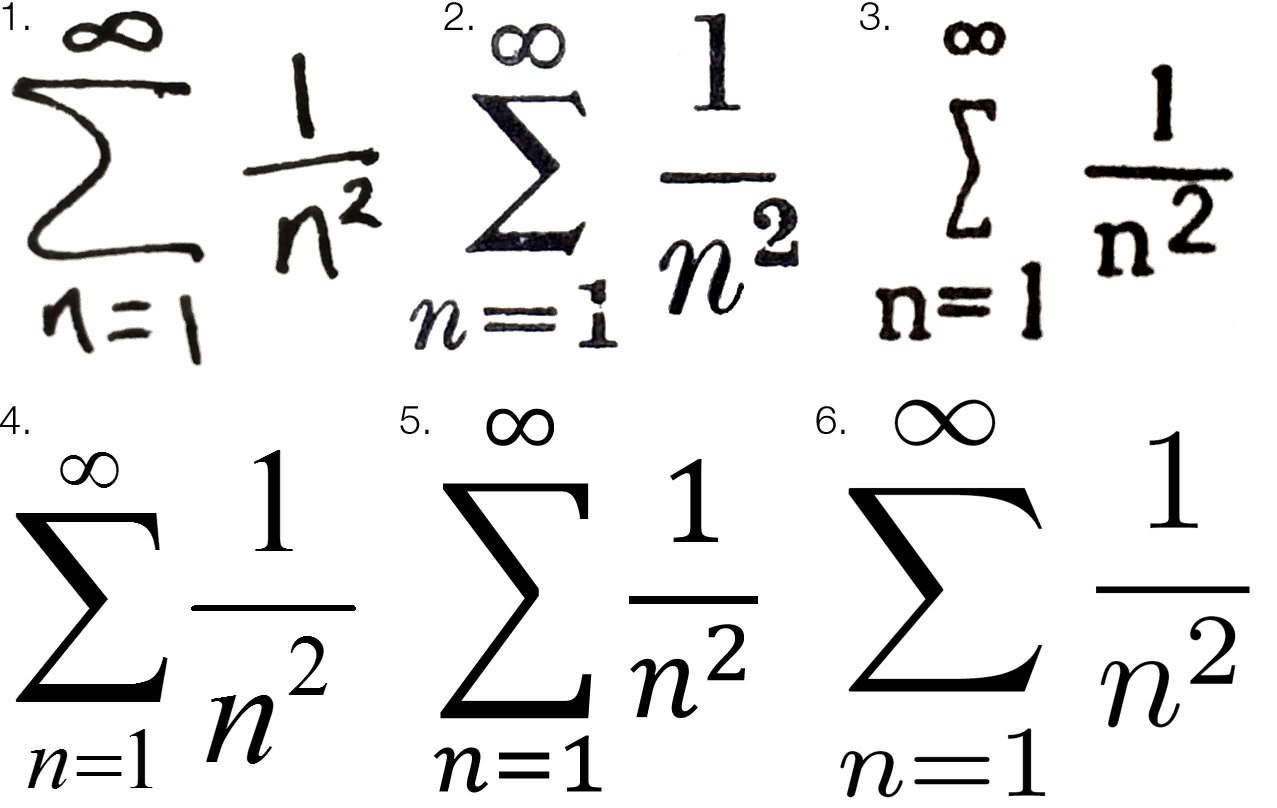
\includegraphics[width=10cm,height=7cm]{gambar/dapi12.jpg}
\begin{equation}Typesetting Math in Latex \end{equation}


 \hspace*{0.5in} Struktur dokumen ini adalah sebagai berikut. Kami memperkenalkan persamaan yang paling dasar di Bagian 2; Bagian 3 kemudian menjelaskan beberapa kemungkinan reaksi pertama ketika sebuah persamaan terlalu panjang Bagian terpenting dari manual ini tercantum dalam Bagian 4 dan 5: disana kita perkenalkan yang bertenaga IEEEeqnarray lingkungan yang harus digunakan masuk apapun bukan meluruskan atau eqnarray.Dalam Bagian 6 beberapa masalah yang lebih maju dan solusi yang mungkin dibahas, dan Bagian 7 berisi beberapa petunjuk dan trik tentang editor Emacs. Akhirnya, Bagian 8 membuat beberapa saran tentang beberapa simbol matematika khusus yang tidak dapat dengan mudah dadjustwidthukan di Latex. \par
\noindent 
perintah akan diatur masuk font mesin tik .RHS berdiri untuk sisi kanan, yaitu, semua istilah di sebelah kanan tanda persamaan (atau ketidaks etaraan).Demikian pula,LHS berdiri untuk sisi kiri, yaitu, semua istilah di sebelah kiri tanda persamaan.Untuk menyederhanakan bahasa kita, kita biasanya akan membicarakannya persamaan. Jelas, typesetting tidak berubah jika sebuah ekspresi sebenarnya adalah ketidaksetaraan. Dokumen ini dilengkapi dengan beberapa file tambahan yang mungkin bisa membantu. \par
\noindent 
 \hspace*{0.5in} Kekuatan utama sebuah LATEX tentang tata bahasa matematika didasarkan pada \par
\noindent 
Paket amsmath. Setiap distribusi SEBUAH LATEX akan datang dengan paket ini \par
\noindent 
disertakan, jadi Anda hanya perlu memastikan bahwa baris berikut disertakan dalam header dokumen anda: \par
\noindent 
\vspace{10pt}
\noindent 
 $  \setminus  $usepackage $  \{  $amsmath $  \}  $ \par
\noindent 
\vspace{12pt}
\noindent 
 $  \setminus  $begin $  \{  $equation $  \}  $ \par
\vspace{12pt}
\noindent 
a = b + c \par
\vspace{12pt}
\noindent 
 $  \setminus  $end $  \{  $equation $  \}  $ \par
\vspace{12pt}
\noindent 
Jika seseorang tidak ingin memiliki nomor persamaan, * -version digunakan: \par
\vspace{12pt}
\noindent 
 $  \setminus  $begin $  \{  $equation* $  \}  $ \par
\vspace{12pt}
\noindent 
a = b + c \par
\vspace{12pt}
\noindent 
 $  \setminus  $end $  \{  $equation* $  \}  $ \par
\vspace{12pt}
\noindent 
Semua kemungkinan lain untuk typesetting persamaan sederhana memiliki kelemahan: \par
\noindent 
  $ \bullet $Itu tampilan matematis lingkungan tidak menawarkan penomoran persamaan. Untuk menambahkan atau re-pindahkan "*" dipersamaan lingkungan jauh lebih fleksibel.
 \par
\noindent 

 Perintah seperti  $  \$  $ $  \$  $ ...  $  \$  $ $  \$  $ , $  \setminus  $ [...  $  \setminus  $], dll, memiliki kelemahan tambahan itu kode sumbernya sangat mudah dibaca. Bahkan,  $  \$  $ $  \$  $ ...  $  \$  $ $  \$  $ salah: Jarak vertikal setelah persamaan terlalu besar dalam situasi tertentu. \par
\vspace{12pt}
\noindent 
\section {Persamaan Tunggal yang Terlalu Panjang: multline} 

\noindent 
 \hspace*{0.5in} Jika sebuah persamaan terlalu panjang, kita harus membungkusnya entah bagaimana. Sayangnya, dibungkus equa-Tions biasanya kurang mudah dibaca daripada yang tidak terbungkus. Untuk meningkatkan keterbacaan, Kita harus mengikuti peraturan tertentu tentang bagaimana melakukan pembungkus: \par
\noindent 

 Secara umum, seseorang harus selalu membungkus sebuah persamaan \par
\noindent 
 Sebelum tanda kesetaraan atau seorang operator \par
\noindent 
 Bungkus sebelum tanda kesetaraan lebih baik dibungkus sebelum operator. \par
Bungkus sebelum operator plus atau minus lebih baik dibungkus sebelum aperkalian-operator \par
\noindent 
 Jenis bungkus lainnya harus dihindari jika memungkinkan.
 \par
\vspace{12pt}
\vspace{12pt}
\noindent 
Cara termudah untuk mencapai pembungkus seperti itu adalah penggunaan \par
\noindent 
multline-lingkungan Hidup: \par
\vspace{12pt}
\noindent 
 $  \setminus  $begin $  \{  $multline $  \}  $ \par
\vspace{12pt}
\noindent 
a + b + c + d + e + f \par
\vspace{12pt}
\noindent 
+ g + h + i \par
\vspace{12pt}
\noindent 
 $  \setminus  $ $  \setminus  $ \par
\vspace{12pt}
\noindent 
= j + k + l + m + n \par
\vspace{12pt}
\noindent 
 $  \setminus  $end $  \{  $multline $  \}  $ \par
\vspace{12pt}
\noindent 
 \hspace*{0.5in} Perbedaannya dengan persamaan lingkungan adalah bahwa break-line sewenang-wenang (atau juga beberapa baris-istirahat) dapat diperkenalkan. Hal ini dilakukan dengan meletakkan a $  \setminus  $ $  \setminus  $ di tempat itu dimana persamaan perlu dibungkus. Demikian pula untuk persamaan* ada juga amultline *-versi untuk mencegah a nomor persamaan Namun, meski mudah digunakan, seringkali IEEEeqnarray lingkungan akan menghasilkan hasil yang lebih baik. Terutama, pertimbangkan situasi umum berikut ini: \par
 
 \begin{verbatim}
\vspace{12pt}
\vspace{12pt}
\noindent 
 $  \setminus  $begin $  \{  $equation $  \}  $ \par
\vspace{12pt}
\noindent 
a = b + c + d + e + f \par
\vspace{12pt}
\noindent 
+ g + h + i + j \par
\vspace{12pt}
\noindent 
+ k + l + m + n + o + p \par
\vspace{12pt}
\noindent 
 $  \setminus  $label $  \{  $eq:equation $ 
  \_  $too $  \_  $long $  \}  $ \par
\vspace{12pt}
\noindent 
 $  \setminus  $end $  \{  $equation $  \}  $ \par
\vspace{12pt}
\vspace{16pt}
\noindent 
Disini RHS terlalu panjang untuk muat di satu baris.
 Itu Multline - lingkungan sekarang akan
  menghasilkan pengikut: \par
\vspace{12pt}
\noindent 
 $  \setminus  $begin $  \{  $multline $  \}
   $ \par
\vspace{12pt}
\noindent 
a = b + c + d + e + f \par
\vspace{12pt}
\noindent 
+ g + h + i + j  $ 
 \setminus  $ $  \setminus  $ \par
\vspace{12pt}
\noindent 
+ k + l + m + n + o + p \par
\vspace{12pt}
\noindent 
 $  \setminus  $end $  \{  $multline $  \}  $ \par
\vspace{12pt}
\vspace{16pt}
\noindent 

\end{verbatim}

 \hspace*{0.5in} Hal ini tentunya jauh lebih baik dari (3), namun memiliki kelemahan yaitu persamaan Tanda kehilangan kepentingannya yang lebih kuat dari operator plus di depan. Lebih baik Solusi disediakan oleh IEEEeqnarray - lingkungan yang akan dibahas secara detail. \par
\vspace{12pt}
\noindent 
\begin{verbatim}


 $  \setminus  $begin $ 
  \{  $IEEEeqnarray $  \}  $ $ 
   \{  $rCl $  \}  $ \par
\vspace{12pt}
\noindent 
a  $  \&  $ =  $  \&  $ b + c + d + e + f \par
\vspace{12pt}
\noindent 
+ g + h + i + j  $  \setminus
  $nonumber $  \setminus  $ $  \setminus  $ \par
\vspace{12pt}
\noindent 
 $  \&  $ $  \&  $ + $  \setminus 
  $> k + l + m + n + o + p \par
\vspace{12pt}
\noindent 
 $  \setminus  $label $  \{  $eq:dont $ 
  \_  $use $  \_  $multline $  \}  $ \par
\vspace{12pt}
\noindent 
 $  \setminus  $end $  \{  $IEEEeqnarray $
   \}  $ \par
\vspace{12pt}
\noindent 
\end{verbatim}
 \hspace*{0.5in} Dalam hal ini baris kedua secara horizontal sejajar dengan baris pertama: + di depan k aku s tepatnya di bawah b , yaitu, RHS jelas terlihat kontras dengan persamaan LHS. Perhatikan juga itu multline salah memaksakan jarak minimum di sebelah kiri yang pertama garis bahkan jika tidak memiliki cukup ruang di sebelah kanan, menyebabkan persamaan yang tidak tersisip. Ini \par
\noindent 
Bahkan bisa mengarah pada tata letak yang sangat jelek dimana baris kedua berisi RHS dari sebuah persamaan sebenarnya ke kiri dari baris pertama yang berisi LHS: \par
\noindent 
 $  \setminus  $begin $  \{  $multline $  \}  $ \par
\vspace{12pt}
\noindent 
a + b + c + d + e + f + g \par
\vspace{12pt}
\noindent 
+ h + i + j  $  \setminus  $ $  \setminus  $ \par
\vspace{12pt}
\noindent 
= k + l + m + n + o + p + q \par
\vspace{12pt}
\noindent 
+ r + s + t + u \par
\vspace{12pt}
\noindent 
 $  \setminus  $end $  \{  $multline $  \}  $ \par
\noindent 
\vspace{16pt}
\noindent 
Sekali lagi ini terlihat jauh lebih baik menggunakan IEEEeqnarray : \par
\vspace{12pt}
\noindent 
 $  \setminus  $begin $  \{  $IEEEeqnarray $  \}  $ $  \{  $rCl $  \}  $ \par
\vspace{12pt}
\noindent 
 $  \setminus  $IEEEeqnarraymulticol $  \{  $3 $  \}  $ $  \{  $l $  \}  $ $  \{  $ $  \%  $ \par
\vspace{12pt}
\noindent 
a + b + c + d + e + f + g \par
\vspace{12pt}
\noindent 
+ h + i + j \par
\vspace{12pt}
\noindent 
 $  \}  $ $  \setminus  $nonumber $  \setminus  $ $  \setminus  $* $  \%  $ \par
\vspace{12pt}
\noindent 
 $  \&  $ =  $  \&  $ k + l + m + n + o + p + q \par
\vspace{12pt}
\noindent 
+ r + s + t + u  $  \setminus  $nonumber $  \setminus  $ $  \setminus  $* \par
\vspace{12pt}
\noindent 
 $  \setminus  $end $  \{  $IEEEeqnarray $  \}  $ \par
\vspace{12pt}
\vspace{12pt}
\noindent 
Kasus 1: Ekspresi bukanlah sebuah persamaan Jika ungkapan itu bukan persamaan, maksudnya, tidak ada tanda kesetaraan, maka tidak ada RHS atau LHS dan multline menawarkan solusi yang bagus: \par
\vspace{12pt}
\noindent 
 $  \setminus  $begin $  \{  $multline $  \}  $ \par
\vspace{12pt}
\noindent 
a + b + c + d + e + f  $  \setminus  $ $  \setminus  $ \par
\vspace{12pt}
\noindent 
+ g + h + i + j + k + l  $  \setminus  $ $  \setminus  $ \par
\vspace{12pt}
\noindent 
+ m + n + o + p + q \par
\vspace{12pt}
\noindent 
 $  \setminus  $end $  \{  $multline $  \}  $ \par
\vspace{12pt}
\noindent 
Kasus 2: Komentar tambaha n Jika ada komentar tambahan di akhir persamaan yang tidak sesuaibaris yang sama, maka komentar ini bisa dimasukkan ke baris berikutnya: \par
\vspace{12pt}
\noindent 
 $  \setminus  $begin $  \{  $multline $  \}  $ \par
\noindent 
a + b + c + d \par
\vspace{12pt}
\noindent 
= e + f + g + h,  $  \setminus  $quad  $  \setminus  $ $  \setminus  $ \par
\vspace{12pt}
\noindent 
 $  \setminus  $text $  \{  $for  $  \}  $ 0  $  \setminus  $le n \par
\vspace{12pt}
\noindent 
 $  \setminus  $le n $  \_  $ $  \{  $ $  \setminus  $textnormal $  \{  $max $  \}  $ $  \}  $ \par
\vspace{12pt}
\noindent 
 $  \setminus  $end $  \{  $multline $  \}  $ \par
\vspace{12pt}
\vspace{16pt}
\noindent 
Kasus 3: LHS terlalu panjang - RHS terlalu pendek Jika LHS dari satu persamaan terlalu panjang dan RHS sangat pendek, maka orang tidak dapat melakukannya Selesaikan persamaan di depan tanda kesetaraan seperti yang diinginkan, tapi seseorang terpaksa melakukannya di suatu tempat di LHS. Dalam hal ini seseorang tidak dapat secara baik menjaga pemisahan alami \par
\noindent 
LHS dan RHS pula dan multline menawarkan solusi yang bagus: \par
\vspace{12pt}
\vspace{12pt}
\noindent 
 $  \setminus  $begin $  \{  $multline $  \}  $ \par
\vspace{12pt}
\noindent 
a + b + c + d + e + f \par
\vspace{12pt}
\noindent 
+ g  $  \setminus  $ $  \setminus  $+ h + i + j \par
\vspace{12pt}
\noindent 
+ k + l = m \par
\vspace{12pt}
\noindent 
 $  \setminus  $end $  \{  $multline $  \}  $ \par
\vspace{12pt}
\noindent 
Kasus 4: Istilah di RHS tidak boleh dibagi Berikut ini adalah kasus khusus (dan agak jarang): LHS akan cukup pendek dan / atau RHS cukup lama untuk membungkus persamaan dengan cara seperti ditunjukkan pada (5), yaitu, ini biasanya akan meminta IEEEeqnarray -lingkungan Hidup. Namun, istilah di RHS adalah sebuah entitas yang kita anggap tidak akan terbelah, tapi terlalu panjang untuk disesuaikan: \par
\vspace{12pt}
\noindent 
 $  \setminus  $begin $  \{  $multline $  \}  $ \par
\vspace{12pt}
\noindent 
h $  \string^  $ $  \{  $- $  \}  $(X $  \vert  $Y)  $  \setminus  $le  $  \setminus  $frac $  \{  $n+1 $  \}  $ $  \{  $e $  \}  $ \par
\vspace{12pt}
\noindent 
- h(X $  \vert  $Y) \par
\vspace{12pt}
\noindent 
 $  \setminus  $ $  \setminus  $ \par
\noindent 
+  $  \setminus  $int p(y)  $  \setminus  $log  $  \setminus  $left( \par
\vspace{12pt}
\noindent 
 $  \setminus  $frac $  \{  $ $  \setminus  $mathsf $  \{  $E $  \}  $ $  \setminus  $bigl[ $  \vert  $X $  \vert  $ $  \string^  $2 \par
\vspace{12pt}
\noindent 
 $  \setminus  $big $  \vert  $ Y=y $  \setminus  $bigr] $  \}  $ $  \{  $n $  \}  $ \par
\vspace{12pt}
\noindent 
 $  \setminus  $right)  $  \setminus  $dd y \par
\noindent 
 $  \setminus  $end $  \{  $multline $  \}  $ \par
\noindent 
Dalam contoh ini integral pada RHS terlalu panjang, tapi tidak boleh dibagi untuk read- kemampuan. Perhatikan bahwa bahkan dalam kasus ini, mungkin saja untuk menemukan solusi berbeda berdasarkan IEEEeqnarray -lingkungan Hidup: \par
\vspace{12pt}
\vspace{12pt}
\noindent 
 $  \setminus  $begin $  \{  $IEEEeqnarray $  \}  $ $  \{  $rCl $  \}  $ \par
\vspace{12pt}
\noindent 
 $  \setminus  $IEEEeqnarraymulticol $  \{  $3 $  \}  $ $  \{  $l $  \}  $ $  \{  $ \par
\vspace{12pt}
\noindent 
h $  \string^  $ $  \{  $- $  \}  $(X $  \vert  $Y) \par
\vspace{12pt}
\noindent 
 $  \}  $ $  \setminus  $nonumber $  \setminus  $ $  \setminus  $ $  \setminus  $quad \par
\vspace{12pt}
\noindent 
 $  \&  $  $  \setminus  $le  $  \&  $  $  \setminus  $frac $  \{  $n+1 $  \}  $ $  \{  $e $  \}  $ \par
\vspace{12pt}
\noindent 
- h(X $  \vert  $Y)  $  \setminus  $nonumber $  \setminus  $ $  \setminus  $ \par
\vspace{12pt}
\noindent 
 $  \&  $ $  \&  $ +  $  \setminus  $int p(y)  $  \setminus  $log  $  \setminus  $left( \par
\vspace{12pt}
\noindent 
 $  \setminus  $frac $  \{  $ $  \setminus  $mathsf $  \{  $E $  \}  $ $  \setminus  $bigl[ $  \vert  $X $  \vert  $ $  \string^  $2 \par
\vspace{12pt}
\noindent 
 $  \setminus  $big $  \vert  $ Y=y $  \setminus  $bigr] $  \}  $ $  \{  $n $  \}  $ \par
\vspace{12pt}
\noindent 
 $  \setminus  $right)  $  \setminus  $dd y \par
\vspace{12pt}
\noindent 
 $  \setminus  $nonumber $  \setminus  $ $  \setminus  $* \par
\vspace{12pt}
\noindent 
 $  \setminus  $end $  \{  $IEEEeqnarray $  \}  $ \par
\vspace{12pt}

\section{Beberapa Persamaan} 
\noindent 
 \hspace*{0.5in} Dalam situasi yang paling umum, kita memiliki urutan beberapa persamaan yang tidak sesuai ke satu baris Disini kita perlu bekerja dengan kesejajaran horizontal untuk menjaga array persamaan dalam struktur yang bagus dan mudah dibaca. Sebelum kami memberikan saran tentang cara melakukannya, kami mulai dengan beberapa buruk contoh yang menunjukkan kelemahan terbesar dari solusi umum. 4.1 Masalah dengan perintah tradisional Untuk mengelompokkan beberapa persamaan, meluruskan -lingkungan Hidup 4 bisa digunakan : \par
\vspace{12pt}
\noindent 
 $  \setminus  $begin $  \{  $align $  \}  $ \par
\vspace{12pt}
\noindent 
a  $  \&  $ = b + c  $  \setminus  $ $  \setminus  $ \par
\vspace{12pt}
\noindent 
 $  \&  $ = d + e \par
\vspace{12pt}
\noindent 
 $  \setminus  $end $  \{  $align $  \}  $ \par
\vspace{12pt}
\noindent 
Sementara ini terlihat rapi asalkan setiap persamaan sesuai dengan satu garis, pendekatan ini tidak Tidak bekerja lagi begitu satu baris terlalu panjang \par
\noindent 
 $  \setminus  $begin $  \{  $align $  \}  $ \par
\vspace{12pt}
\noindent 
a  $  \&  $ = b + c  $  \setminus  $ $  \setminus  $ \par
\vspace{12pt}
\noindent 
 $  \&  $ = d + e + f + g + h + i \par
\noindent 
  \par
\noindent 
+ j + k + l  $  \setminus  $nonumber $  \setminus  $ $  \setminus  $ \par
\vspace{12pt}
\noindent 
 $  \&  $ + m + n + o  $  \setminus  $ $  \setminus  $ \par
\vspace{12pt}
\noindent 
 $  \&  $ = p + q + r + s \par
\vspace{12pt}
\noindent 
 $  \setminus  $end $  \{  $align $  \}  $ \par
\vspace{12pt}
\noindent 
Disini + m harus di bawah d dan tidak di bawah tanda kesetaraan. Tentu saja, bisa saja tambahkan beberapa spasi, misalnya,  $  \setminus  $ hspace  $  \{  $... $  \}  $ , tapi ini tidak akan pernah menghasilkan pengaturan yang tepat (dan gaya pemrograman yang buruk!). Solusi yang lebih baik ditawarkan oleh eqnarray -lingkungan Hidup \par
\vspace{12pt}
\noindent 
 $  \setminus  $begin $  \{  $eqnarray $  \}  $ \par
\vspace{12pt}
\noindent 
a  $  \&  $ =  $  \&  $ b + c  $  \setminus  $ $  \setminus  $ \par
\vspace{12pt}
\noindent 
 $  \&  $ =  $  \&  $ d + e + f + g + h + i \par
\vspace{12pt}
\noindent 
+ j + k + l  $  \setminus  $nonumber $  \setminus  $ $  \setminus  $ \par
\vspace{12pt}
\noindent 
 $  \&  $ $  \&  $ + $  \setminus  $> m + n + o  $  \setminus  $ $  \setminus  $ \par
\vspace{12pt}
\noindent 
 $  \&  $ =  $  \&  $ p + q + r + s \par
\vspace{12pt}
\noindent 
 $  \setminus  $end $  \{  $eqnarray $  \}  $ \par
\noindent 
\vspace{16pt}
\noindent 
Itu eqnarray -lingkungan Hidup, 5 Namun, memiliki beberapa kelemahan yang sangat parah: \par
\noindent 
 Ruang di sekitar tanda-tanda kesetaraan terlalu besar. Terutama, memang begitu tidak itu sama seperti di multline – dan persamaan lingkungan: \par
\vspace{12pt}
\noindent 
 $  \setminus  $begin $  \{  $eqnarray $  \}  $ \par
\vspace{12pt}
\noindent 
a  $  \&  $ =  $  \&  $ a = a \par
\vspace{12pt}
\noindent 
 $  \setminus  $end $  \{  $eqnarray $  \}  $ \par
\vspace{12pt}
\noindent 
Ungkapan kadang tumpang tindih dengan angka persamaan meski ada akan cukup ruang di sebelah kiri: \par
\vspace{12pt}
\noindent 
 $  \setminus  $begin $  \{  $eqnarray $  \}  $ \par
\vspace{12pt}
\noindent 
a  $  \&  $ =  $  \&  $ b + c \par
\noindent 
 $  \setminus  $ $  \setminus  $ \par
\vspace{12pt}
\noindent 
 $  \&  $ =  $  \&  $ d + e + f + g + h $  \string^  $2 \par
\vspace{12pt}
\noindent 
+ i $  \string^  $2 + j \par
\vspace{12pt}
\noindent 
 $  \setminus  $label $  \{  $eq:faultyeqnarray $  \}  $ \par
\vspace{12pt}
\noindent 
 $  \setminus  $end $  \{  $eqnarray $  \}  $ \par
\vspace{12pt}
\noindent 
Itu eqnarray lingkungan menawarkan sebuah perintah  $  \setminus  $ lefteqn  $  \{  $... $  \}  $ yang bisa digunakan ketika LHS terlalu panjang: \par
\noindent 
\vspace{16pt}
\noindent 
 $  \setminus  $begin $  \{  $eqnarray $  \}  $ \par
\vspace{12pt}
\noindent 
 $  \setminus  $lefteqn $  \{  $a + b + c + d \par
\vspace{12pt}
\noindent 
+ e + f + g + h $  \}  $ $  \setminus  $nonumber $  \setminus  $ $  \setminus  $ \par
\vspace{12pt}
\noindent 
 $  \&  $ =  $  \&  $ i + j + k + l + m \par
\vspace{12pt}
\noindent 
 $  \setminus  $ $  \setminus  $ \par
\vspace{12pt}
\noindent 
 $  \&  $ =  $  \&  $ n + o + p + q + r + s \par
\vspace{12pt}
\noindent 
 $  \setminus  $end $  \{  $eqnarray $  \}  $ \par
\noindent 
\vspace{16pt}
\noindent 
Sayangnya, perintah ini salah: jika RHS terlalu pendek, arraynya tidak terpusat dengan benar \par
\noindent 
\vspace{16pt}
\noindent 
 $  \setminus  $begin $  \{  $eqnarray $  \}  $ \par
\vspace{12pt}
\noindent 
 $  \setminus  $lefteqn $  \{  $a + b + c + d \par
\vspace{12pt}
\noindent 
+ e + f + g + h $  \}  $ \par
\vspace{12pt}
\noindent 
 $  \setminus  $nonumber $  \setminus  $ $  \setminus  $ \par
\vspace{12pt}
\noindent 
 $  \&  $ =  $  \&  $ i + j \par
\vspace{12pt}
\noindent 
 $  \setminus  $end $  \{  $eqnarray $  \}  $ \par
\vspace{12pt}
\noindent 
Apalagi sangat rumit untuk mengubah kesejajaran horizontal dari persamaan tanda di baris kedua.  \par
\vspace{12pt}
\noindent 
Solusi:~penggunaan dasar IEEEeqnarray Itu IEEEeqnarray  Lingkungan adalah perintah yang sangat kuat dengan banyak pilihan. DiManual ini kami hanya akan memperkenalkan beberapa fungsi yang paling penting. Untuk informasi lebih lanjut kami lihat manual resmi Pertama-tama, agar bisa menggunakan IEEEeqnarray Lingkungan, seseorang perlu memasukkan paketnya IEEEtrantools Sertakan baris berikut di header dokumen Anda: \par
\vspace{12pt}
\vspace{12pt}
\noindent 
 $  \setminus  $usepackage $  \{  $IEEEtrantools $  \}  $ \par
\vspace{12pt}
\noindent 
Kekuatan IEEEeqnarray adalah kemungkinan menentukan jumlah kolom dalam array persamaan Biasanya, spesifikasi ini akan jadi  $  \{  $rCl $  \}  $, yaitu tiga kolom, yaitu Kolom pertama benar-dibenarkan, yang tengah berpusat dengan sedikit ruang lebih banyak t (oleh karena itu kita tentukan kapital C bukan huruf kecil c) dan kolom ketiga dibiarkan dibenarkan: \par
\vspace{12pt}
\noindent 
 $  \setminus  $begin $  \{  $IEEEeqnarray $  \}  $ $  \{  $rCl $  \}  $ \par
\vspace{12pt}
\noindent 
a  $  \&  $ =  $  \&  $ b + c \par
\vspace{12pt}
\noindent 
 $  \setminus  $ $  \setminus  $ \par
\vspace{12pt}
\noindent 
 $  \&  $ =  $  \&  $ d + e + f + g + h \par
\vspace{12pt}
\noindent 
+ i + j + k  $  \setminus  $nonumber $  \setminus  $ $  \setminus  $ \par
\vspace{12pt}
\noindent 
 $  \&  $ $  \&  $ + $  \setminus  $> l + m + n + o \par
\vspace{12pt}
\noindent 
 $  \setminus  $ $  \setminus  $ \par
\vspace{12pt}
\noindent 
 $  \&  $ =  $  \&  $ p + q + r + s \par
\vspace{12pt}
\noindent 
 $  \setminus  $end $  \{  $IEEEeqnarray $  \}  $ \par
\vspace{12pt}
\vspace{16pt}
\noindent 
 \hspace*{0.5in} Namun, kita bisa menentukan jumlah kolom yang dibutuhkan. Sebagai contoh,  $  \{  $c $  \}  $ akan memberi saja satu kolom (yang terpusat) atau  $  \{  $rCl "l $  \}  $akan menambahkan kolom keempat yang dibenarkan kiri itu bergeser ke kanan (jaraknya ditentukan oleh "), misalnya untuk spesifikasi tambahan.Apalagi disamping l,c,r,L,C,R untuk entri mode matematika, ada juga s,t,kamu untuk kiri, tengah, dan kanan. Dan spasi tambahan bisa jadi ditambahkan oleh. Dan /dan ? dan "dalam rangka meningkatkan ketertiban. 8 Rincian lebih lanjut tentang penggunaan IEEEeqnarrayakan diberikan di Bagian 5. Perhatikan bahwa berbeda dengan eqnarray ruang di sekitar tanda-tanda persamaan benar. \par
\vspace{12pt}
\noindent 
\section {Sebuah komentar tentang konsistensi} 
Ada tiga isu lagi yang belum disebutkan sejauh ini, tapi itu mungkin penyebabnya ketidakkonsistenan saat ketiga lingkungan tersebut, persamaan, \par
\noindent 
multline, dan IEEEeqnarray, digunakan secara intermixedly: \par
\noindent 
 multline memungkinkan sebuah persamaan dimulai dari atas halaman, sementara persamaan dan IEEEeqnarray cobalah untuk meletakkan garis teks terlebih dahulu, sebelum persamaan dimulai. Bahkan, jarak sebelum dan sesudah lingkungan tidak persis sama persamaan,multline, dan IEEEeqnarray. \par
\noindent 
  $ \bullet $persamaan menggunakan mekanisme otomatis untuk memindahkan nomor persamaan keBaris berikutnya jika ungkapannya terlalu panjang. Sementara ini nyaman, terkadang nomor persamaan dipaksa ke baris berikutnya, meski masih ada cukup ruang tersedia di telepon: \par
  \begin{verbatim}
  
 
\vspace{20pt}
\vspace{20pt}
\noindent 
 $  \setminus  $begin $ 
  \{  $equation $  \}  $ \par
\vspace{12pt}
\noindent 
a =  $  \setminus  $sum $ 
 \_  $ $  \{  $k=1 $  \}  $ $  
 \string^  $n $  \setminus  $sum $  
 \_  $ $  \{  $ $  \setminus  $ell=1 $  \}  $ $  \string^  $n \par
\vspace{12pt}
\noindent 
 $  \setminus  $sin  $  
 \setminus  $bigl(2 $  \setminus  $pi  $ 
  \setminus  $, b $  
 \_  $k  $  \setminus  $, \par
\vspace{12pt}
\noindent 
c $  \_  $ $  \{  $ $ 
 \setminus  $ell $  \}  $  $ 
  \setminus  $, d $  \_  $k  $

  \setminus  $, e $  \_  $ $  \{  $ $  \setminus  $ell $ 
 \}  $  $  \setminus  $, \par
\vspace{12pt}
\noindent 
f $  \_  $k  $  \setminus  $, g $
  \_  $ $  \{  $ $  \setminus  $ell $  \}  $  $  \setminus  $, h  $  \setminus  $bigr) \par
\vspace{12pt}
\noindent 
 $  \setminus  $end $ 
  \{  $equation $  \}  $ \par
\vspace{12pt}
\noindent 
Dengan IEEEeqnarray penempatan nomor
 persamaan sepenuhnya berada
  di bawah kontrol: \par
\vspace{12pt}
\noindent 
 $  \setminus  $begin $ 
  \{  $IEEEeqnarray $  \}  $ $ 
   \{  $c $  \}  $ \par
\noindent 
a =  $  \setminus  $sum $ 
 \_  $ $  \{  $k=1 $  \}  $ $ 
  \string^  $n $  \setminus  $sum $  
\_  $ $  \{  $ $  \setminus  $ell=1 $ 
 \}  $ $  \string^  $n \par
\noindent 
 $  \setminus  $sin  $ 
  \setminus  $bigl(2 $ 
   \setminus  $pi  $  
   \setminus  $, b $ 
  \_  $k  $  \setminus  $, \par
\noindent 
c $  \_  $ $  \{  $ $  
\setminus  $ell $  \}  $  $ 
 \setminus  $, d $  \_  $k  $  
\setminus  $, e $  \_  $ $ 
 \{  $ $  \setminus  $ell $ 


 \}  $  $  \setminus  $, \par
\noindent 
f $  \_  $k  $  \setminus  $, g $ 
 \_  $ $  \{  $ $ 
  \setminus  $ell $ 
   \}  $  $
  \setminus  $, h  $ 
   \setminus  $bigr) \par
\noindent 
 $  \setminus  $IEEEeqnarraynumspace \par
\noindent 
 $  \setminus  $label $ 
  \{  $eq:labelc1 $  \}  $ \par
\noindent 
 $  \setminus  $end $ 
  \{  $IEEEeqnarray $  \}  $ \par
\noindent 
\vspace{12pt}
\noindent 
\vspace{12pt}
\noindent 
Atau \par
\noindent 
\vspace{12pt}
\noindent 
 $  \setminus  $begin $  
 \{  $IEEEeqnarray $  \}  $ $ 
  \{  $c $  \}  $ \par
\noindent 
a =  $  \setminus  $sum $ 
 \_  $ $  \{  $k=1 $  \}  $ $ 
  \string^  $n $  \setminus  $sum $ 
   \_  $ $  \{  $ $  
   \setminus  $ell=1 $ 
    \}  $ $  \string^  $n \par
\noindent 
 $  \setminus  $sin  $ 
  \setminus  $bigl(2 $  \setminus 
   $pi  $  \setminus  $, b $  \_  $k 
    $  \setminus  $, \par
\noindent 
c $  \_  $ $  \{  $ $  \setminus 
 $ell $  \}  $  $  \setminus  $, d $  
 \_  $k  $  \setminus  $, e $  
 \_  $ $  \{  $ $ 
 
  \setminus  $ell $  \}  $  $  
  \setminus  $, \par
\noindent 
f $  \_  $k  $  \setminus  $, g $  \_  $ $  \{  $ $  \setminus  $ell $ 
 \}  $  $ 
 \setminus  $, h  $  \setminus  $bigr) \par
\noindent 
 $  \setminus  $nonumber $ 
  \setminus  $ $  \setminus  $* \par
\noindent 
 $  \setminus  $label $  \{  $eq:labelc2 $  \}  $ \par
\noindent 
 $  \setminus  $end $  \{  $IEEEeqnarray $  \}  $ \par
\noindent 
\vspace{12pt}
\noindent 
 \end{verbatim}

Jika ini tidak diinginkan, seseorang dapat mengubah perilaku IEEEeqnarray Berperilaku seperti persamaan:  $  \setminus  $ renewcommand  $  \{  $ $  \setminus  $ theequationdis $  \}  $  $  \{  $ $  \{  $ $  \setminus  $ normalfont ( $  \setminus  $ theequation) $  \}  $ $  \}  $  $  \setminus  $ renewcommand  $  \{  $ $  \setminus  $ theIEEEsubequationdis $  \}  $  $  \{  $ $  \{  $ $  \setminus  $ normalfont ( $  \setminus  $ theIEEEsubequation) $  \}  $ $  \}  $ \par
\vspace{12pt}
\noindent 
 $  \setminus  $textbf $  \{  $ $  \setminus  $textit $  \{  $ $  \setminus  $color $  \{  $red $  \}  $ \par
\noindent 
This is our main result: \par
\noindent 
 $  \setminus  $begin $  \{  $IEEEeqnarray $  \}  $ $  \{  $rCl $  \}  $ \par
\noindent 
a  $  \&  $ =  $  \&  $ b + c  $  \setminus  $ $  \setminus  $ \par
\noindent 
 $  \&  $ =  $  \&  $ d + e  $  \setminus  $IEEEyesnumber \par
\noindent 
 $  \setminus  $IEEEyessubnumber \par
\noindent 
 $  \setminus  $end $  \{  $IEEEeqnarray $  \}  $ $  \}  $ $  \}  $ \par
\noindent 
\vspace{12pt}

